\documentclass[a4paper]{article}
\usepackage[letterpaper, margin=1in]{geometry} % page format
\usepackage{listings} % this package is for including code
\usepackage{graphicx} % this package is for including figures
\usepackage{amsmath}  % this package is for math and matrices
\usepackage{amsfonts} % this package is for math fonts
\usepackage{tikz} % for drawings
\usepackage{hyperref} % for urls
\usepackage{pdfpages}

\title{Final Exam}
\author{Max Schemitsch}
\date{5/13/2019}

\begin{document}
\lstset{language=Python}

\maketitle

\section{Problem 1}
\subsection{(c)}
Using $final.SVM.sinc.py$ with $N=1000$, the best hyper-parameters I obtained were $C=512$, $\epsilon = 0$, $\gamma = 0.5$, and CV Score $= 0.410219$.


\begin{figure}[h]
  \begin{center}
    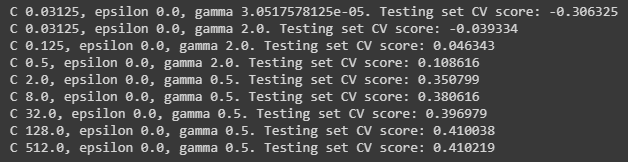
\includegraphics[width=150mm,scale=1]{problem1c.png}
  \end{center}
\end{figure}


\subsection{(d)}
We can interpret the results in a few ways.


It can be seen that as $C$ increases, both Gamma and CV Score also increase. Throughout my various runs of the program, the CV Score ended up being negative for all cases where $C=0.03125$. Only when $C$ was equal to $0.125$ and up did the CV Score become positive. It's hard to tell if there's a relationship between $C$ and $\epsilon$ as my epsilon value never changed.


Based on how the hyper-parameters are displayed, it seems that $C$ is similar to a neural network layer, as we see multiples of 2 like 8, 32, 128, and 512. I'm not sure what epsilon is, as the only value I obtained is 0. Gamma seems to be sort of like a ETA or learning speed, as lower gammas give better CV scores, but the gamma value never gets too low.
\newpage


We can also look at the plot produced in the second half of $final.SVM.sinc.py$:


\begin{figure}[h]
  \begin{center}
    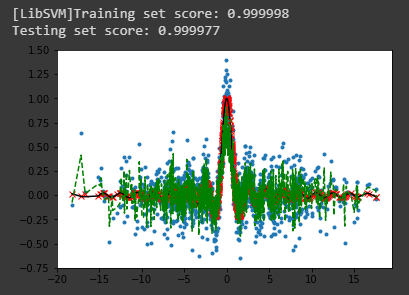
\includegraphics[width=80mm,scale=0.8]{problem1d.png}
  \end{center}
\end{figure}


We can see that the both our training and testing scores are basically 100\%. The plot also tells us that the SVR predictions were roughly accurate to the model, especially on the bump in the middle.


\subsection{(e) (extra credit)}

Using $N=10000$ we can see similar results to before. After a few unsuccessful attempts, running the code for an roughly an hour produced my best $C=0.125$, $\epsilon=0$, $\gamma=2$, and CV Score $= 0.285745$.

\begin{figure}[h]
  \begin{center}
    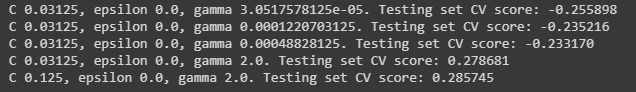
\includegraphics[width=150mm,scale=1]{problem1e.png}
  \end{center}
\end{figure}


Our plot is similar to before, but noticeably populated with more sample predictions.


\begin{figure}[h]
  \begin{center}
    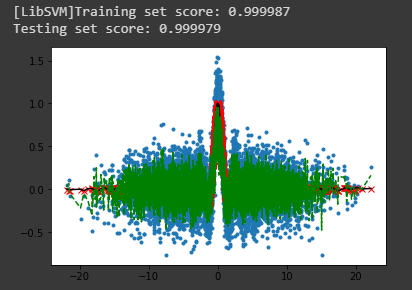
\includegraphics[width=80mm,scale=1]{problem1e2.png}
  \end{center}
\end{figure}


\newpage


\section{Problem 2}
\subsection{(b) \& (c)}
Using the code in $final.SVM.dig.py$, the best set of hyper-parameters were $C=256$, $\epsilon = 1.6$, $\gamma = 0.0625$, and CV Score $= 0.335753$. These was the best set of values I obtained. The 500 or so iterations following this set all produced values will less CV Score.


\begin{figure}[h]
  \begin{center}
    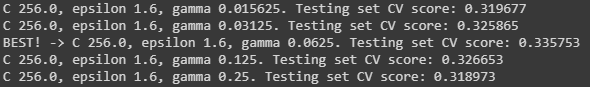
\includegraphics[width=150mm,scale=1]{problem2b.png}
  \end{center}
\end{figure}


In terms of patterns, it seems that the best gamma level is 0.0625. Many of my new best scores used this gamma value, and at glance value it seems this way too for most combinations of $C$ and epsilon. I'm going to guess that perhaps $C=256$ is one of the best options for $C$ values, as I didn't get a new best CV for 512, 1024, 2048, etc. In fact it seems like CV Scores never approached the 0.335XXX mark again after $C$ reached 1024. The best epsilons varied, as earlier with $C=64$ they ranged in between 0.6 and 0.9, but afterwards tended to be in the 1.5 to 1.7 range.


We also produce a plot. To get this plot working I had to change a bit of code as it was perhaps outdated:


\begin{lstlisting}[frame=single]
cmap = cm.get_cmap("Spectral")
for i in range(X_te.shape[0]):
  plt.text(X_te[i, 0], X_te[i, 1], str(y_te[i]), 
  color=cmap(round(ypred[i]) / 10.), 
  fontdict={'weight': 'bold', 'size': 9})
\end{lstlisting}


This allows the spectral function to work, and results in this plot:


\begin{figure}[h]
  \begin{center}
    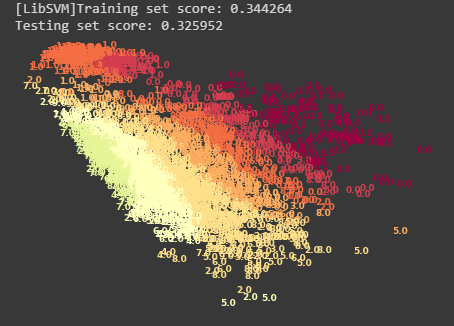
\includegraphics[width=100mm,scale=1]{problem2b2.png}
  \end{center}
\end{figure}


A few things can be noted from this chart; firstly, the training and testing scores are both close to the iterated CV Scores we obtained earlier. We can also see that the predictions are separated into colors by ranges. The deep reds and light reds hover around 0 and 1, and lighter colors have a wider range of values. To be frank, I'm not sure how to interpret this graph, but it seems that with values closer to 1 or 0, testing and training scores seem to be better.


\newpage


\subsection{(d) (extra credit)}
The Colaboratory file is called $MaxSchemitsch\_DATA440\_FinalExam.ipnyb$. It combines both $final.SVM.dig.py$ and $final.SVM.sinc.py$. It also contains the minor adjustments I made for the $Spectral$ issue. I added headers and was going to add comments, but the code was already commented so I wasn't sure what to put. To use the notebook, one still has to upload $finalGenData.py$, $finalGetDigits.py$, $features.csv$, and $features-t.csv$.
\end{document}